%%% Thesis Introduction --------------------------------------------------
\chapter{INTRODUCTION}
\label{chap:intro}
\graphicspath{{Introduction/IntroductionFigs/EPS/}{Introduction/IntroductionFigs/}}
\nomenclature[z1]{\cms}{Character Motion Synthesis}
\nomenclature[z2]{\cpg}{Central Pattern Generator}
\nomenclature[z3]{\dof}{Degree of Freedom}

\section{The Challenge}
Character Motion Synthesis (\cms) research aims at generating motion for virtual characters.
It is a valuable topic for both industry and academic community. 
Besides major applications in the media industry, where both computer games and animation films depend heavily upon character motion for storytelling;  
CMS also has applications in many different areas, such as user interface design, psychology, sports and medicine.

The challenge of \cms research is not to make characters move, but how to make them lifelike. 
Underneath this challenge is human's marvellous ability of motion perception. 
In fact, motions are very similar; 
while from the varieties in motion details, humans can infer the changes in mental states, health conditions or the surrounding environment.
\note{uncanny valley}
A famous phenomon of motion perception characteristics is the ``uncanny valley''.
For characters with realistic humanlike appearance, slightly artefacts in motions may result a big drop in human likeness.



Nowadays in industry, high quality motions are mainly generated by manual work. 
In applications,characters are very complex and contain a large number of joints, making animation tedious work.
Making it worse, reusing motion animation is also difficult and prone to artefacts.
High level animation tools are badly needed. 

\note{Do An introduction for physicall based animaiton?}
Physics based \cms is the current research endeavor.
The expectation is the elimination of the artefacts that violate physics laws and interactive dynamic responses to environmental perturbations.
Currently,this paradigm faces many difficulties including computational cost and modelling complexity.
Same problems has been identified by biological researchers from different perspectives.

The ``uncanny valley '' prompts us the percetion question of dynamics.
Motion is not judged by validity of physics.
Some awkward artefacts are spotted instantly even they are physically feasible, while many physical impossible motions are accepted as realistic and entertaining. 

How we perceive the world is fundamental to how we move through it.
The peculiarity of motion perception and control suggests a different principle is adopted by the neural system.
Difficulties in \cms reflects the inferiority of artificial control.
By exploring new biological research , this thesis proposes a different approach.

 

\section{Agile Animals}
%\note{Underlying these problems} is our misunderstanding of animal motions.
Although motions of animals have fascinated us for thousands of years, we still don't fully understand how they move.
Animals are very different from artificial machines.
Investigations into such differences provide an in-depth understanding of problems of \cms researche.
%some basic questions of motor control and motion perception remain open. 
%And answers to such questions become even more valuable nowadays. 
%Advance in this topic will greatly influence the biology, robotic engineering even intelligent research.
\note{The difference between biological motor system}

%The paradoxes is even human are good at motor control and motion perception; human still don’t have an idea of how we move and how we perceive motion.
%Before going into details into the research ideas, we first review some puzzles troubles the foundation of CMS. 
\begin{itemize}
\HiItem {Degrees of freedom ({\dof}s)}.
From Mechanical perspective, animals have many more {\dof}s than their artificial counterparts.
An artificial ship can be approximated by a simple rigid body; while the flexible vertebrae of fishes has tens of {\dof}s.


In principle, the extra {\dof}s admit more types of motion variations. 
But from the control perspective, the extra {\dof}s complicate the control problem. 
For a human to take one step,  the neural system controls more than 600 muscles .
Extra {\dof}s are redundant and become the ``{\dof}s Curse'' for motor control.
 
\HiItem {Versatility}
Most artificial machines are designed with a single purpose,while animals are capable  of unlimited motion tasks.
For human, beside the walking, swimming and many other styles of locomotion , human motion behaviour involves lots of tools, such as cars, skate, bicycle, and tennis.
Some behaviours often negalected by \cms research such as the feeding, breeding, language, vision depend on motor control. 
What follows is the question of how many resources are allocated for motor control.

It seems much following traditional control approach but biologicalresearch shows very little.

\HiItem{Performance}
Although for animals,  motor control is more complex , the resulting performance surpasses artificial machines in many aspects.
Natural motion are more
\begin{enumerate} 

\HiItem{Robust:}
Human can maintain walking stability on tough terrain unaccessible for vehicles.

\HiItem{Maneuverable and speed:}
Typical modern airplanes will travel $32\: body\: lengths/sec$ and yaw $720\: deg/sec$ at max.
while pigeons may travel $75 \:body\: length / sec$, yaw at about more than $5000deg/sec$.

\HiItem{Energy Efficient:}
The energy consumed by human walking is only $5\%$ of that for the world famous humanoid ASIMO.
\end{enumerate}

\end{itemize}



%For computer animation research, the key principle is we should know the things we animate.
%Natural motion system has many valuable properties which are not captured by current motion synthesis methods.
%\begin{itemize} 
% \HiItem{robust}
%Natural motions are adaptive to the changes in the environment or body conditions. 
%A common example is human locomotion. 
%Walking on different terrains will exhibit different gait while the balance is maintained. 
%
%\HiItem{speedy}
%Some motions of animals are very fast, honey birds may vibrate their wings in kHz.
%The astonishment is to the speed of motion, more puzzling is that the neural system can solve the complex motion control problem in such a short time. 
%When an animal avoids obstacles at very high running speed, 
%it must continue its running, make a turning and keep balance at the same time. 
%It seems easy for the neural system to plan complicate motions.
%\HiItem{Energy Efficient}
%Natural Motions are energy efficient.
%In theory, this idea is supported by Darwin's Theory of Evolution.
%But animals spent far less energy than our expectation.
%An example is that the energy consumed by human walking is only 5\% of that for a robot of the same scale.
%\end{itemize}

\section{Motor Invariant Theory}

The approach proposed in this thesis is different from current \cms methods .
A side by side comparison will highlight the distinction and novelity. 

\subsection{Major Differences}
\begin{itemize}
\HiItem {Control Function Model}
The procedural approach support computational model of motor control.
It is the redundant {\dof}s that spoil this approach  with inhibitive computational cost.
Pure procedural methods are impossible to run in real-time.

As an alternative, some researchers support the memory based model for motor control and have developed data-driven methods.
But such methods lacks the versatility and adaptivity.
Unlimited memory for data is needed and searching in ever increasing database becomes more and more challenging.

The foudation of the new approach is that motions are ``easy'' and need little control effort.
It is the body and environment that play the crucial role, their dynamic interaction form the basic templates for motor control.
The neural system only tweaks the basic templates for specific purpose.



 
 
	
\HiItem{Control Strategy}
Most artificial control methods follow the principle of feedback.
The motion trajectory is planned first and control is applied to counteract perturbations.
This method is also called ``continuous shooting''.


The control strategy in the new approach is feed forward.
The strategy is to make motions ``easier''.
If perturbations can be predicted, measures are taken beforehand to prevent ``failure''.
Thus motion trajectory is unconrolled, only the final result is of concern.


\HiItem{Natural Dynamics} 
Many \cms methods plan the motion trajectory before execution.
The natural dynamics of the body and environment are treated as perturbations and are canceled by the control input.


The mechanical structures of animals have evolved with the enivronment for millions of years, in the process of natural selection.
They are advantages rather than hanicap. 
The new approach limit the control input and explore the natural dynamics for the natural-looking features.
\end{itemize}


\subsection{Motor Invariant Theory}
%In this thesis, we propose different idea towards motor control and motion synthesis.
%In this research, we propose a different motion synthesis method based on a different motor control theory.
%
%An insightful discovery is that motor control can be “easy”.
%For some situation, some tasks mainly explore the properties of the body and environment and can be achieved with little control effort.
%In nature, we don’t finish difficult motion tasks, we select many easy motion tasks that we are good at, connect or modify them for our special purpose.
%
%The “easy” tasks are called motion primitives; they are the basic elements of our motor ability. 
%When we modify the motion primitives, some valuable properties of motion primitives are kept unchanged, and the maintained properties are called motor invariants.
%
%The inspiration of our idea comes from related biological research, which covers biomechanics and neural science.
To make new ideas workable, new mathematical tools are introduced to develope control techniques.
At the center of the new theory is the mathematical modelling of the motion templates and the ``tweaking'' exerted by the neural system.
The insightful discovery is that when motion adapts, certain properties of natural dynamics are maintained, which called motor invariants.
The new theory of motor control is the motor invariant theory:
\begin{itemize}

\item Qualitatively, the property of ``easiness'' should be maintained.
Structural Stability arises as an abstraction of the intuitive idea of ``easiness''.
Motion adaptations are modelled as topological conjugations. 

\item For the quantitative properties, we explore the idea of ``Symmetry''.
Lie Groups are introduced to model the ``tweaking'' actions that maintain the local quantative properties.


\item More complex tasks are executed by combining simple tasks together.
The basic motion tasks are called motion primitives, of which the number is limited.
For an animal, the repetorie of motion primitives is determined by the body and environment.
\end{itemize}

Although new mathematical tools seems obscure at first glimpse.
The ideas behind are intuitive and can be explained well by commonly observed phenomena.



\subsection{The Floating Ship: An example of Stability}
We use the floating ship as an example to show the relation between ``easiness'' and topological conjugacy.
In real life, ships floating on the wave, are typically taller than they are wide,as shown in Figure~\ref{fig:ShipFloating}.
The  question is how the ship maintain its posture.

Through analyzing the qualitative dynamic properties, we see that maintaining posture is trival.
This conclusion applies to different ships are their dynamics are topological equivalent.


\begin{figure}[!htbp]
  \begin{center}
    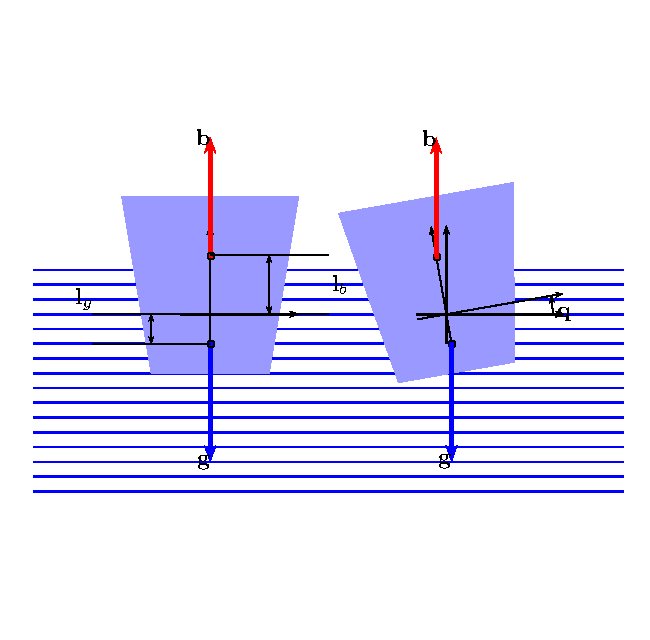
\includegraphics{ShipExample}
    \caption{The Floating Ship Example}
    \label{fig:ShipFloating}
  \end{center}
\end{figure}

\subsubsection*{Dynamics}
The sway motion shown in Figure ~\ref{fig:ShipFloating} is described by Equation~\ref{eq:shipflow}
\begin{equation}
\label{eq:shipflow}
J\ddot{q}+d\dot{q}=\tau(q)_{g}+\tau(q)_{b}+\tau_{u}
\end{equation}

$q$ is the swaying angle.
$J$ is the inertia,  
$d$ is the damping coefficient,
$\tau_{g}$,$\tau_{b}$,$\tau_{u}$ are the coresponding the torques of gravity, buoyancy and external control.
When $\tau_{u}=0$,  the floating ship  becomes an \emph{autonomous system} governed by natural dynamics and.

To make it consistent with discussions in following chapters, Equation~\ref{eq:shipflow} is reformulated.
Define the \emph{state} variable $\state=[q,\qd]$, new form is
\[
\dot{\state}=F_{J,d}(\state)+Du
\]

wheren 
$F$ is a function of $\state$, the subscripts~$J$ and~$d$ are \emph{system parameters}.
$D$ is a matrix,which describe how the control effort is applied.
$u$ is \emph{control input}, for this example is $\tau_{u}$



\subsubsection*{Equilibrium Postures}
A ship will only rest when $\tau_{g}+\tau_{b}+\tau_{u}=0$, which are called \emph{Equlibrium} Postures.
For the ship, the only two possible ones are show in Figure ~\ref{fig:ShipEqulibrium}
\begin{figure}[!htbp]
  \begin{center}
     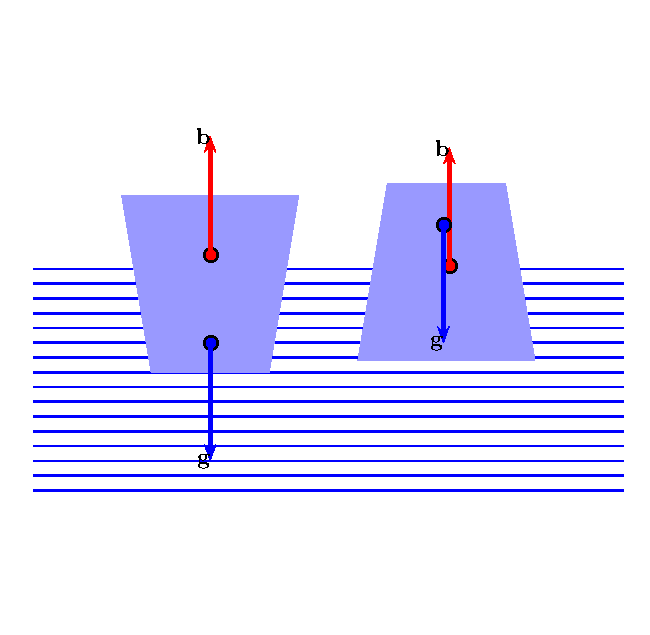
\includegraphics{ShipEquilibrium}
    \caption{The Stable and Unstable Equilibrium Posture}
    \label{fig:ShipEqulibrium}
  \end{center}
\end{figure}



The two postures are different, illustrated with the \emph{phase plot}.
On the phase plot, the horizontal axis represents the sway angle $q$; and the vertical axis for the angle velocity $\qd$. 
The motion of the ship is shown as a curve on the phase plot, which is called \emph{flow}.

The left posture is \emph{attractive} or \emph{stable}.
If a small perturbation moves the ship away from the left posture, it will return to the equilibrium posture automatically as shown in Figure~\ref{fig:StablePosture}.
\begin{figure}[!htbp]
  \begin{center}
      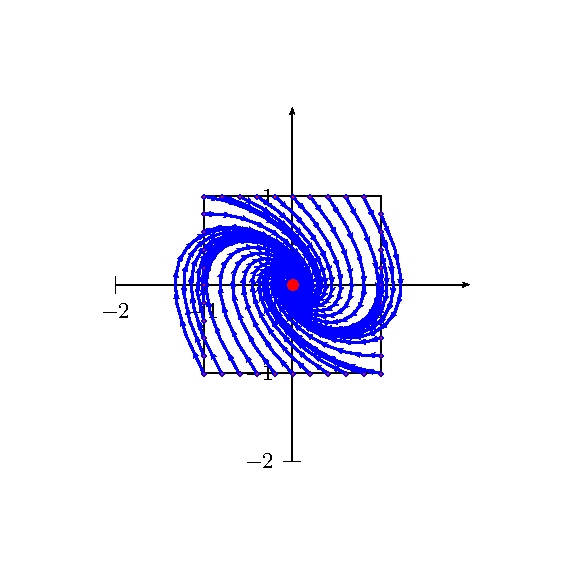
\includegraphics{stablePosition}
    \caption{Phase Plot of the Stable Posture}
    \label{fig:StablePosture}
  \end{center}
\end{figure}


The right posture is \emph{repelling} or \emph{unstable}.
Away from the equilibrium posture, it will move away further, as shown in Figure~\ref{fig:unStablePosture}.

\begin{figure}[!htbp]
  \begin{center}
      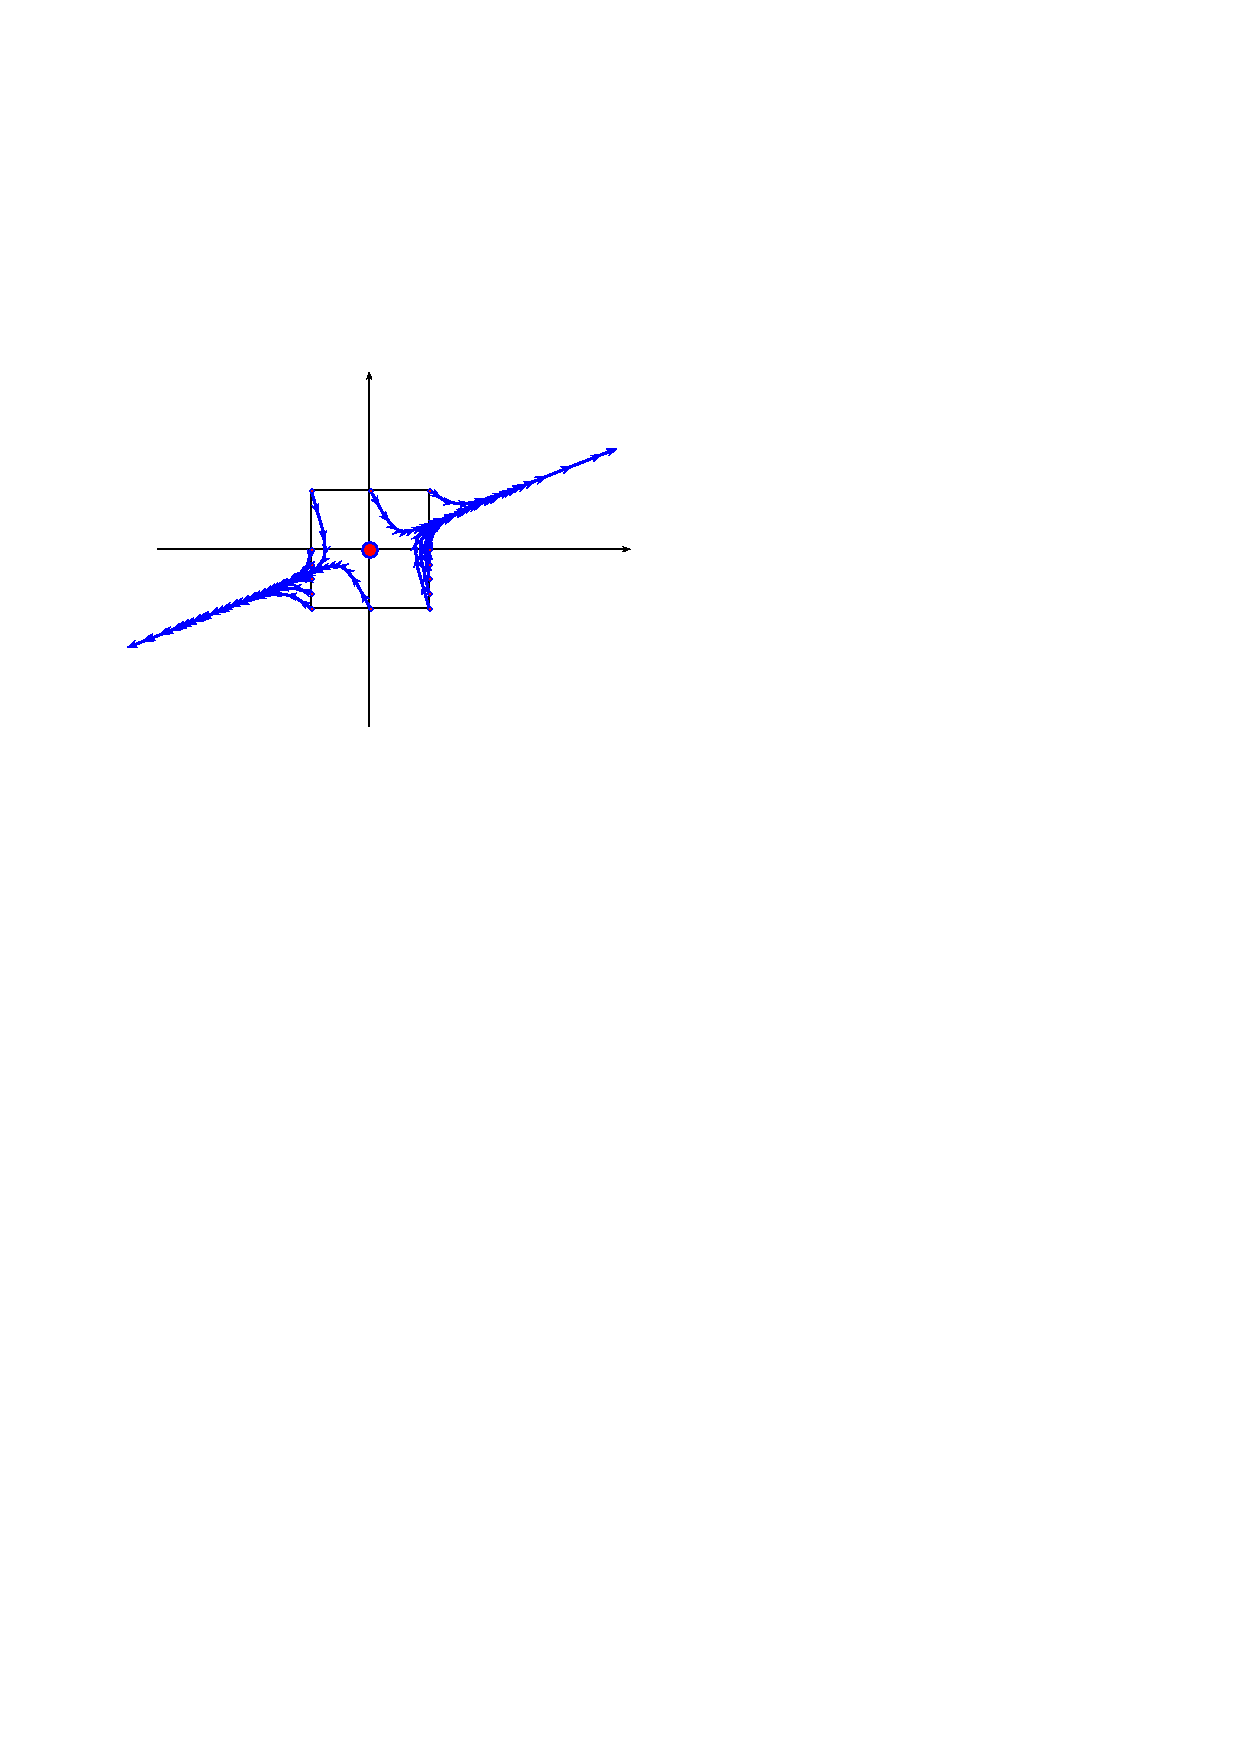
\includegraphics{unstablePosition}
    \caption{Phase Plot of the Unstable Posture}
    \label{fig:unStablePosture}
  \end{center}
\end{figure}


\subsubsection*{``Easiness''}
All the flows form the \emph{phase portrait} of the floating ship system. 
The discovery is that all the flows start from the repelling posture and ends at the attractive posture.
Several example curves are show in Figure ~\ref{fig:globalflow}

This means the left posture is maintain by the natural dynamics, the balancing task is trival.
For the ship, this property is determined by structure design (the center of bouyancy is above the center of gravity).

\begin{figure}[!htbp]
  \begin{center}
   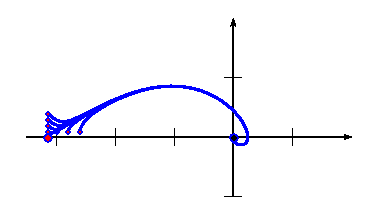
\includegraphics[width=0.7\textwidth]{ShipGlobalFlow}
   \caption{Global Properties of the Flows: All the curves starts from the repelling posture(Red) and ends at the attractive one(Blue)}
   \label{fig:globalflow}
  \end{center}
\end{figure}

 



\subsubsection*{Generalization of the Ship Example} 
This conclusion is independent of the shape, size, weight or material. 
Same wave perturbations will result in different sway motions for different ships.
As long as the qualitative structure design criteria is maintained, balancing is ``easy''.
On phase portraits,  all the ships share following properties. 
\begin{itemize}
\item one repelling point 
\item one attractive point 
\item all flows starts from repelling point and ends at the  attractive point. 
\end{itemize}


\begin{figure}[!htbp]
  \begin{center}
   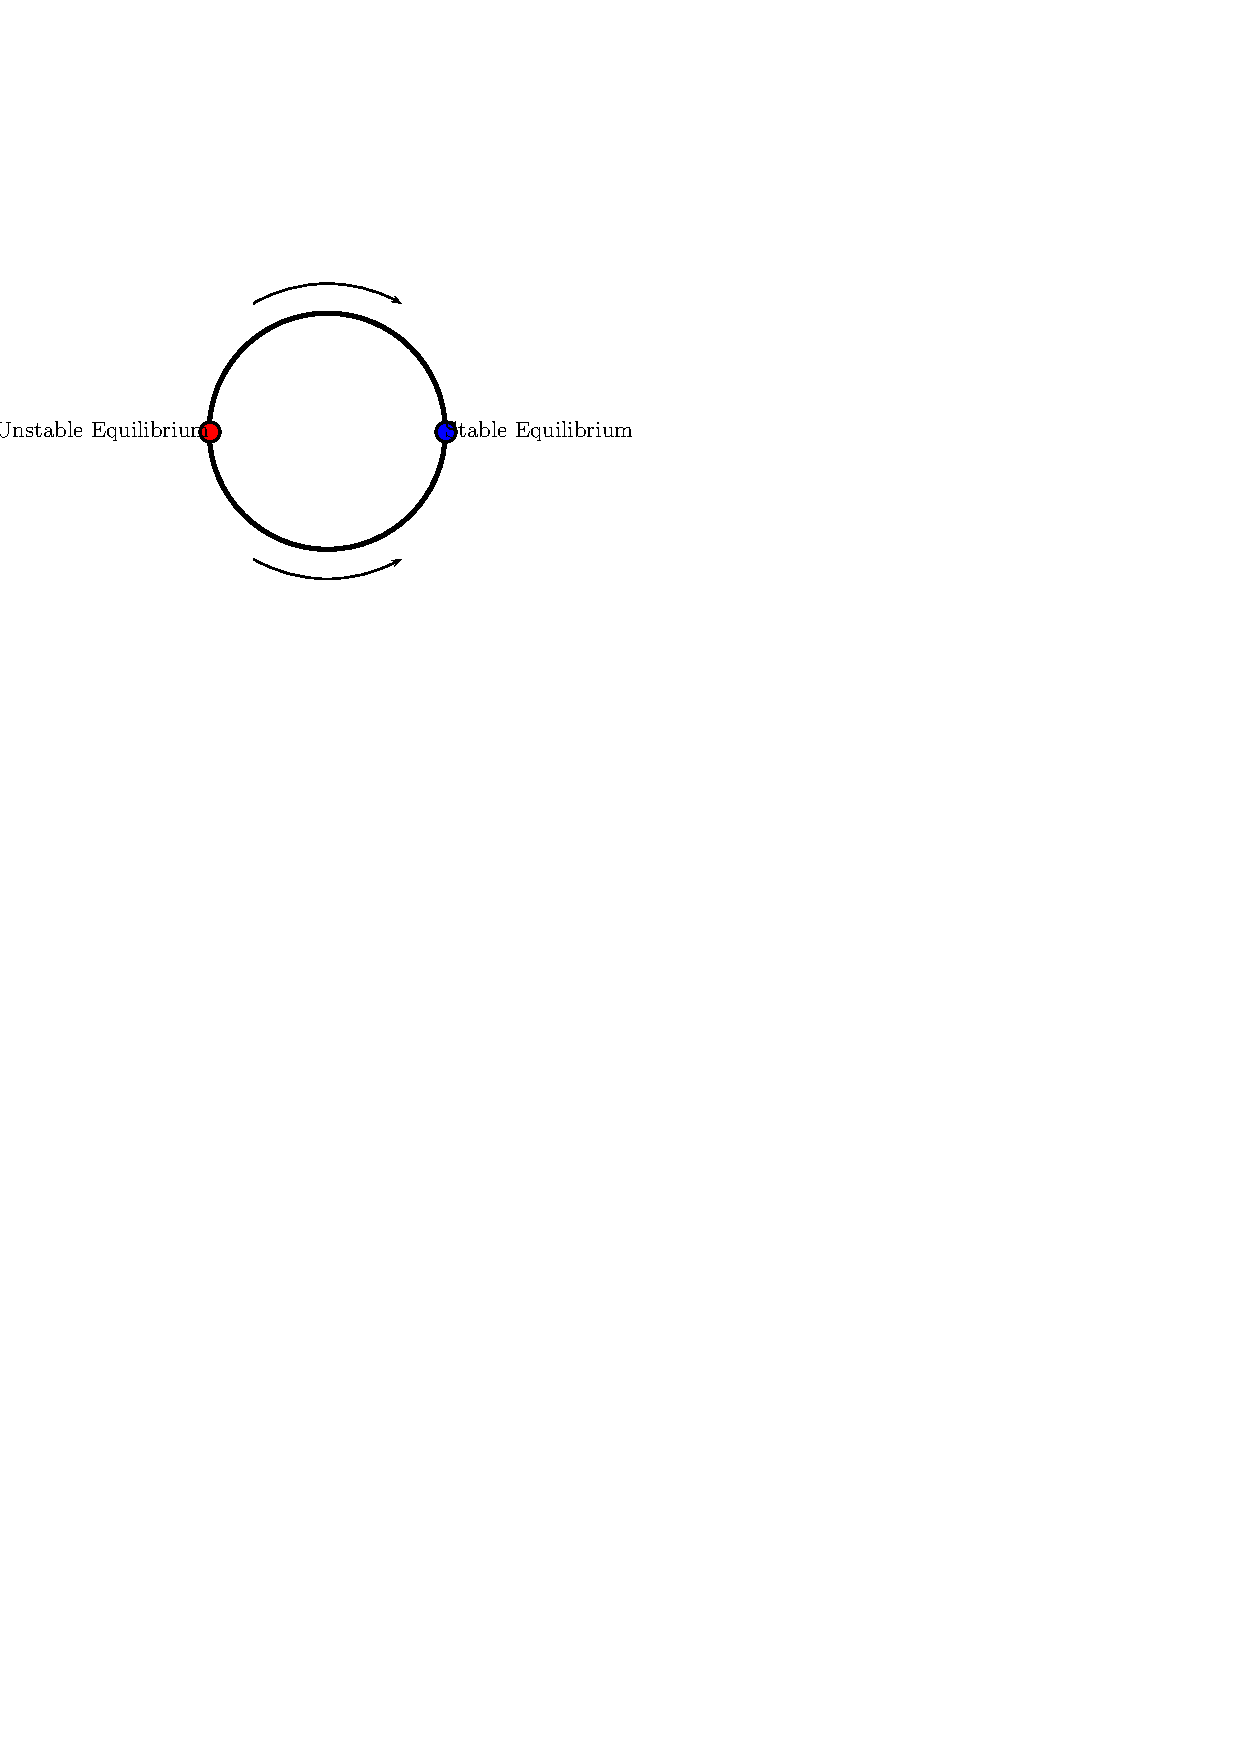
\includegraphics{topologyStructure}
   \caption{The Toplogy Structure of the phase portraits of Floating Ship System}
   \label{fig:topologyStructure}
  \end{center}
\end{figure}



These properties are qualitative or \emph{topological}.
The phase portraits of different ships share the topological structure in Figure~\ref{fig:topologyStructure}.
Two ships  $\dot{\state}=F(\state)$ and $\dot{\state}=F^{'}(\state)$ are topological equivalent, or more specifically \emph{topology conjugate}.

This relationship is presented by $F \simeq F'$.
$F$ and $F'$ are called \emph{analogous systems}.


In Motor Invariant Theory, the topological structure is one important motor invariant: the \emph{Global Motor Invariant}.
Global motor invariant determines the ``easiness'' or stability of motions.
Adaptations geerated by adjusting system parameters are \emph{System Adaptations}


\subsection{The Mass Spring System: A system with Symmetry}
Despite the complexity of body structure, motions of animals are executed with high accuracy in real-time.
Real-time accuracy in motor control is another puzzle, as solving the complex dynamics requires inhibitative computational cost.

To this end, Lie Group Theory is introduced in Motor invariant theory, 
quantative properties control explores the idea of ``Symmetry''; new motions are transformed from some templates.

This ideas of symmetry and transformation  can be illustrated by the following mass spring example.
The mass spring system in Figure~\ref{fig:massspring} captures some important properties of biological natural dynamics.
The muscle actuators are compiliant and works like spring and  bones are represented by mass.

\begin{figure}[!htbp]
  \begin{center}
    \includegraphics[width=0.7\textwidth]{MassSpring}
    \caption{the mass spring system}
    \label{fig:massspring}
  \end{center}
\end{figure}

\subsubsection*{Dynamics}




The canonical equation of mass spring system is

\begin{equation}
\label{eq:mass-spring}
\ddot{q}+q=0.
\end{equation}

by define the \emph{state variable}, $\state=[q,\qd]$, it can also be reformulated as
\[
\dot{\state}=F(\state)
\]

and corresponding phase plot of two flows is Figure~\ref{fig:massSpringPhasePlot}.


\begin{figure}[!htbp]
\label{fig:massSpringPhasePlot}  
  \begin{center}
     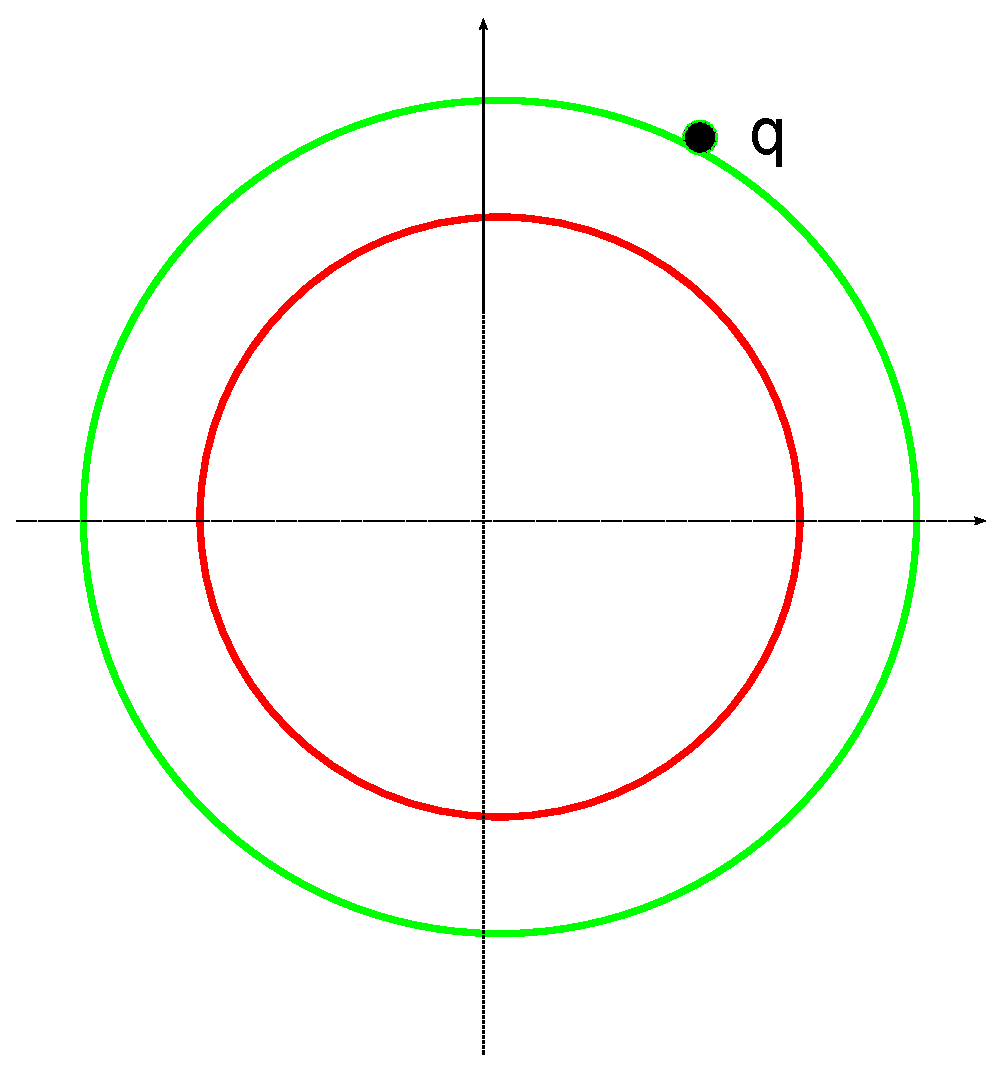
\includegraphics[width=0.5\textwidth]{MassSpringPhasePlot}
    \caption{Mass Spring Phase Plot:two motion curves are shown.The red one and the green pass through different state $\state$,$\state^{'}$}
  \end{center}
\end{figure}

\subsubsection*{Symmetry and Transformation}
It is highly unlikely animals can solve Equation~\ref{eq:mass-spring}.

the mass spring system has some ``symmetrical properties''.
Different flows share the same circle ``Shape''.
New flows(green) can be find by scaling the original(red) flow.

From mechanical viewport, this is because the flows of mass spring are energy perserving.
we can define the energy function
\[
E=\frac{1}{2}(m\qd^2+kq^2)
\]
when $m=1,k=1$, $E=constant$ means $q^2+\qd^2=constant$, which is the implicit function of a circle.

Given flows that pass through  $\state$.
For the state $\state^{'}$, by checking the energy, the scale transformation from red to green can be workout,then we know the future motion after $\state^{'}$.


\subsubsection*{Dynamic Perception}
the Impact of ``transformation and symmetry'' idea reaches beyond motor control. 
Besides reducing the computational costs, it also suggests a real-time perception mechansim.
The dynamics can be encoded in a different manner in brain: a motion template and the symmetry propety of the system.
We check whether the observed motion(green) can be transformed from our memorized motions (red).
If so, motion are accepted as realistic, otherwise artefacts are detected.


\subsubsection*{Local Motor Invariant and Transform Adaption}
To verify the symmetry properties of motion, it is unnecessary to work out the transformation. 
We can just check the properties invariant under transformation.
For the mass spring system example, we can check the ``the shape'' or whether current motion is energy perserving. 
From differential geometrical perspective,  the curvature is invariant. 


Quantitative invariant properties like energy perserving or curvature of flow are called \emph{Local Motor Invariant}. 
Adaptation generated by transformation is called \emph{transform adaptation}.

\section{Contribution}
\emph{Global Motor Invariant} captures the qualitative properties while \emph{Local Motor Invariant} determines quantitative properties. 
In Motor Invariant Theory,  Neural system preserve certain motor invariants according to the motion purpose. 

Motion Adaptation is achieved through \emph{System Adaptation} and \emph{Transform Adaptation}.

Compared with current \cms methods, the new approach has several advantages:
\begin{enumerate}
\HiItem {More sytles of motion adaptation}
Compared with traditional dynamics \cms methods,\emph{System Adaptation} and \emph{Transform Adaptation} generate more types of adaption in motion style.
\HiItem {Better usability}.
Adaptation motion is more easy. 
Artists  adjust  parameters according their purpose, other motion properties are automatically perserved.
\HiItem {Computationally Efficient} 
This motion synthesis approach runs in real-time.
\HiItem {Motion Transition}
Dynamic motion transiton are developed with the solid theory foundation.
\HiItem {No Reference Motion}
This dynamic method requires no motion data.

\end{enumerate}

For the method is based on the bioligical principle of motor control, but the methodology is different.
Usually new  theories of motor control are developped by analytical methodology.
This approach is simulation based and new mathematical tools introduced my shed light into biology reseawrch, and can be treated as theorical candidates that needs further research proof.

\begin{enumerate}
\item Motion Primitive is an old idea in biological research. 
Currently methods identify motion primitives based on empirical statisics and machine learning.

Motor Invarian Theory is more complete.
Besides identifification, it also answers why certain motions are primitives and others are not,
how many motion primitives we have and where they come from.

\item For the neural structrue \cpg , their roles on adjust motions are well agreed.
While concrete strategy for adjust \cpg parameters according to motor purpose is still lacking.
In the motor invariant theory,  such a strategy is developed.

\item For perception research, motion and dynamic perception mechanism of neural system is still unclear.
The motor invariant theory propose a computationally efficient mathematical machinery.

\item Synergy in muscle actuation is identify by emprical methods. 
The `` control symmetry '' method work in the ``synergy manner''  and can treated an explainationary theory.
\end{enumerate}







\section{Organization of the Thesis}

This thesis is organized as follows.
 
In Chapter~\ref{chap:background}, previous research on motion synthesis and biological motor control are discussed, which are the motivation and justification of motor invariant theory.
 
In Chapter~\ref{chap:gi}, \emph{Global Motor Invariant} and qualitative property of motion are discussed. 
Differential topology is introduced to analyze the qualitative properties.
Biological based  methods for maintaining the global motor invariant are developed.

Chapter~\ref{chap:li} focuses on the idea of Local Motor Invariant and Symmetry.
Lie Group Theory is  introduced  to analyze the symmetry properties in motion dynamcs.
Symmetry Controllers are developed for adaptation motions.
 


Chapter~\ref{chap:msf} discuss the combination problems.
For each motion primitive,  strategies are developed to preserve global and local motor invairant simutaneously.
Motion primitive transition is dicussed as the theory of combining motion elements into more complex motion.
As an animation system, the software architecture and work flow are discussed at the end.

Chapter~\ref{chap:gi},~\ref{chap:li},~\ref{chap:msf} lay the theoretical foundation for the motion synthesis control and is treated as the Motion Invariant Theory.
Following chapters focus on application of this theory to generate animations.



Chapter~\ref{chap:walk}, focuses the tweaking of one primitive.
Bipedal walking is chosen, which is one of the most challenging problem for current \cms research.
Motor Invariant Theory introduce method to boost the stability and generate adaptive gaits.


In Chapter~\ref{chap:stance}, combinations of motion primitives are discussed.
A new balancing motion primitive is developed. 
Transitional motions are generated for stance to walk and walk to stance transitions.

In Chapter~\ref{chap:highdor}, extensions of motor invariant theory to more complex characters are discussed.
Three different strategies are developed for different situations.

This thesis ended with Chapter~\ref{chap:con}. 
After dicussion of new finding of this research, some new question and ideas for graphics and neural science are proposed for further research .





%%% ----------------------------------------------------------------------


%%% Local Variables: 
%%% mode: latex
%%% TeX-master: "../thesis"
%%% End: 

